% Adapted from the PGF shapes.multipart manual's rectangle-split example.
\documentclass[border=2pt]{standalone}
\usepackage{tikz}
\usetikzlibrary{shapes.multipart}
\begin{document}
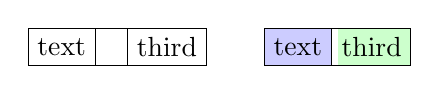
\begin{tikzpicture}[every node/.style={draw,anchor=text,rectangle split,rectangle split horizontal,rectangle split parts=3}]
  \node {text \nodepart{two} \nodepart{three}third};
  \node[rectangle split ignore empty parts,rectangle split part fill={blue!20,red!20,green!20}] at (3,0)
    {text \nodepart{two} \nodepart{three}third};
\end{tikzpicture}
\end{document}
